\documentclass[a4paper,12pt]{article}
\usepackage[utf8]{inputenc}
\usepackage[top=2cm, bottom=2cm, left=3cm, right = 1.5cm]{geometry}
\usepackage[T2A]{fontenc}
\usepackage[english,russian]{babel}
\usepackage{amsmath,amsfonts,amstext,amssymb}
\usepackage{graphicx}
\bibliographystyle{plain}
\usepackage{xfrac}
\usepackage{multicol}
\setlength{\columnsep}{0.8pt}
\sloppy
\title{Учет неразрешенных двойных при оценивании массы рассеянных звездных скоплений}


\author{О. И. Бородина$^1$ \and А. Ф. Селезнев$^1$ \and Дж. Карраро$^2$ \and В. М. Данилов$^1$ }

\date{\footnotesize{
    $^1$ Уральский Федеральный Университет, ул. Мира 19, Екатеринбург\\%
    $^2$ Dipartimento di Fisica e Astronomia, Universita’ di Padova Vicolo Osservatorio 3, Padova, Italy}\\% 
    }


\begin{document}
\maketitle
\section*{Реферат}
Одна из проблем, с которой сталкиваются исследователи звездных скоплений при оценивании их массы по функции светимости, это наличие в скоплении неразрешенных двойных систем. Особенно важно учитывать это обстоятельство при исследовании рассеянных звездных скоплений, где доля двойных может составлять десятки процентов. Цель настоящей работы -- оценить, насколько учет неразрешенных двойных систем изменяет массу скопления.
 
В этой работе мы использовали функции светимости рассеянных звездных скоплений IC 2714, NGC 1912, NGC 2099, NGC 6834 и NGC 7142, которые были получены методом звездных подсчетов в ходе работы над созданием однородного каталога структурных и динамических характеристик рассеянных звездных скоплений по данным каталога точечных источников 2МАSS.

\section*{Введение}
Первые упоминания факта о наличии в звездных скоплениях большого количества неразрешенных двойных звезд можно обнаружить в работе Haffner \& Heckmann (1937) \cite{HH}.
С тех пор наличию двойных звезд было посвящено множество различных исследований. Например, Maeder в 1974 \cite{Maeder} показал, как располагается двойная на диаграмме звездная величина - показатель цвета в зависимости от отношения масс компонет $q=M_2/M_1$ (где $M_2$ это масса вторичной компоненты, а $M_1$ -- масса главной компоненты двойной). В своей работе Hurley \& Tout (1998) \cite{HT} продемонстрировали, что последовательность, которая лежит выше главной последовательности звезд скопления на диаграмме CMD, образована двойными. Причем авторы этой работы выяснили, что коэффициент q имеет широкий разброс значений, то есть отношение масс компонент двойной может быть различным и может быть не равно 1 (что соответствует случаю одинаковых масс). 

Доля двойных звезд в шаровых звездных скоплениях относительно мала и обычно не превышает десяти процентов \cite{Milone2012} за несколькими исключениями. Однако, в работе Li с соавторами \cite{Li17} были обнаружены три шаровых скопления с гораздо большей долей двойных $(0.6-0.8)$

Рассеянные звездные скопления имеют значения доли двойных $\alpha \geqslant 30\%$ \cite{Li17, Boni, Khalaj, Sarro, alPer}. Этот процент все же меньше чем доля двойных среди звезд в окрестностях Солнца \cite{Duq1}. Было также получено, что доля двойных растет с увеличением массы главного компонента. Это чаще всего связано с динамической эволюцией звездного скопления \cite{KOP,Dorval}.

Очень важной характеристикой является функция распределения отношения масс компонент двойной $q$. В настоящее время среди исследователей нет точного согласия по поводу формы этого распределения. Согласно работе Duquennoy \& Mayor за 1991 год \cite{Duq2} функция распределения имеет максимум ближе к случаю маломассивных вторичных компонент, то есть далеко от 1. И наоборот, есть работы (например у Fisher с соавторами \cite{Fisher}), где пик расположен около случая равных масс компонент. Такой же пик был  обнаружен Maxted и другими \cite{Maxted} для маломассивных спектральных двойных в молодых скоплениях около $\sigma Ori$ и $\lambda Ori$. В работе Reggiani \& Meyer \cite{RM} была получена универсальная форма для распределения параметра $q$ для звезд типа Солнца и для карликов класса М в поле: $dN/dq \sim q^{\beta}$ с $\beta=0.25\pm0.29$. Это распределение можно считать плоским внутри интервала ошибок. 

Milone \cite{Milone2012} с соавторами определил, что  в интервале $q\in[0.5,1.0]$ распределение параметра $q$ у шаровых скоплений примерно плоское, с некоторыми отклонениями для нескольких случаев. А в работе Kouwenhoven и др. \cite{Kouwenhoven} использовались два других распределения: степенная зависимость $dN/dq \sim q^{\beta}$ для $q\in[q_0,1]$ и различных $\beta$, и Гауссово $dN/dq \sim exp[-(q-\mu_q)^2/2\sigma_q]$ для $q\in(0,1]$ с $\mu_q=0.23$ and $\sigma_q=0.42$.

Распределение отношения масс компонент двойной является ключом к восстановлению характеристик первоначальной популяции двойных. Было проведено множество численных исследований в данном направлении \cite{Kroupa2011,Geller2013,PR}.

Geller  и его соавторы \cite{Geller2013} показали на модели N-тел скопления NGC188, что распределение орбитальных параметров короткопериодичных двойных типа Солнца (с $P<1000^d$) должно быть примерно неизменным даже в пределах миллиарда лет эволюции. Это значит, что современные наблюдения двойных даже в старых скоплениях могут дать необходимую информацию о первоначальной их популяции. Parker \& Reggiani \cite{PR} показали, что общая доля двойных уменьшается в ходе динамической эволюции, но форма распределения $q$ не изменяется.  

Наличие неразрешенных двойных звезд в звездных скоплениях искажает оценки массы ЗС. Это следует учитывать как в случае звездных подсчетов, так и при оценке динамической массы (по значению дисперсии скоростей). Если набор звезд, отобранных по  оценке дисперсии скоростей (через лучевые скорости) содержит спектроскопические двойные, то значение дисперсии скоростей будет завышено. В результате, это приведет к завышенному значению массы скопления.

В работах Bianchini с соавторами \cite{Bianchini} и Kouwenhoven \& de Grijs \cite{KdeG} был сделан вывод, что учет населения двойных при оценке массы скопления очень важен. Селезнев с соавторами \cite{4337} отметили возможное влияние неразрешенных двойных на дисперсию скоростей, а затем и на оценку массы скопления NGC 4337.

Когда масса скопления определяется через функцию светимости, полученную методом звездных подсчетов, то оценка массы будет меньше, чем в реальности, если не учитывать наличие в ЗС неразрешенных двойных. Это может быть легко объяснено тем, что масса двойной звезды больше массы одиночной с той же звездной величиной из-за сильной зависимости светимости звезд от их массы ($(L/L_{\odot})\sim(M/M_{\odot})^4$ \cite{CO}). 
Если одиночная звезда имеет ту же звездную величину, что и двойная, то их светимости также равны $L_s=L_1+L_2$ (где $L_s$ -- светимость одиночной звезды, а  $L_1$ и $L_2$ - светимости главного и вторичного компонента двойной соответственно). Тогда $M_s^4=M_1^4+M_2^4$, а значит $(M_1+M_2)^4=M_1^4+M_2^4+4M_1M_2^3+6M_1^2M_2^2+4M_1^3M_2=M_s^4+4M_1M_2^3+6M_1^2M_2^2+4M_1^3M_2$.
 Так как все величины положительные, то $(M_1+M_2)^4>M_s^4$, и $M_1+M_2>M_s$.
 
 Наличие неразрешенных двойных было учтено в работе Khalaj \& Baumgardt (2013) \cite{Khalaj} для оценки массы РЗС Ясли. Авторы определили долю двойных в скоплении -- $30\pm5$ процентов, а затем нашли поправочный коэффициент, равный 1.35 (чтобы учесть неразрешенные двойные в скоплении, следует умножить массу скопления, полученную в предположении, что все звезды в нем одиночные, на данный множитель). 
К сожалению, Khalaj \& Baumgardt \cite{Khalaj} не объяснили, каким образом был получено значение этого множителя. 

Сейчас мы планируем новый проект, который будет включать в себя оценки масс достаточно большого количества РЗС при помощи функции светимости. Тем самым, интересно выполнить оценку того, как корректирующий множитель зависит от доли двойных $\alpha$ и распределения $q$ в довольно большом интервале значений этих параметров. Это и является целью настоящей работы.

Она организована следующим образом: сначала  описывается принятая модель и используемый алгоритм, затем приводится описание и анализ результатов для пяти РЗС NGC 1912, NGC 2099, NGC 6834, NGC 7142, и IC 2714. 
	
	\section*{Модель и алгоритм}
Поправочный коэффициент к массе скопления зависит от двух параметров. Во-первых, необходимо учитывать распределение доли двойных по звездным величинам. В данном исследовании мы используем равномерное распределение, то есть доля двойных звезд одинакова для всех звездных величин, и имеет значения в интервале $10-90 \%$
Во-вторых, распределение параметра q может быть различным, в данной работы мы рассматриваем несколько видов распределений:
\begin{itemize}
	\item $\delta$ - функцию с $q = 1$
	\item плоское распределение
	\item Гауссово распределение из работы Kouwenhoven и др. \cite{Kouwenhoven}
	\item Гауссово распределение с модой, сдвинутой ближе к 1, чтобы воспроизвести результаты из работ Fischer и др. \cite{Fisher} и Maxted и др. \cite{Maxted}.
\end{itemize}

Математическое ожидание и стандартное отклонение последнего распределения имеют следующие значения: $\mu_q=0.60$ и $\sigma_q=0.42$.

Ранее уже рассматривали решения задач, связанных с моделированием двойных систем. Обзор таких работ был сделан Kouwenhoven \cite{Kouwenhoven} с соавторами и включает в себя следующие варианты постановки задач:

\begin{itemize}
	\item Случайное моделирование пары. Массы обоих компонентов случайным образом выбирается из распределения масс;
	\item Случайное моделирование пары, ограниченной главным компонентом. Масса главного компонента выбирается из распределения масс, затем выбирается масса звезды-спутника с требованием, чтобы она была меньше;
	\item Моделирование пары, ограниченный главным компонентом. Масса главного компонента выбирается из распределения масс, затем вычисляется масса звезды-спутника из распределения параметра $q$.;
	\item Расщепление ядра. Общая масса двойной системы берется из распределения масс. Масса главного компонента и звезды-спутника вычисляются по формулам связи массы системы и параметра $q$.
\end{itemize}
Наша задача отличается от решенных ранее, так как нам дана изначально звездная величина двойной системы, из которой мы должны определить массу компонентов. Таким образом, метод, описанный ниже, может быть назван <<моделированием пары, ограниченной общей светимостью>>.

Для того, чтобы связать массу и звездную величину, мы используем квадратичную функцию масса-светимость \ref{EkersEq} из работы Eker и др. \cite{Eker}:

\begin{equation}
\begin{array}{l}
\log{L} = - (0.705 \pm 0.041)(\log{M})^2  + (4.655 \pm 0.042) (\log {M}) - (0.025 \pm 0.010)\\
\label{EkersEq}
\end{array}
\end{equation}
где $L$ -- это светимость, выраженная в единицах светимости Солнца, а $M$  -- масса звезды, выраженная в массе Солнца.
 В своей работе Eker \cite{Eker} с соавторами получили еще и другие виды зависимостей, а также привели ряд аргументов, показывающих преимущество использования именно квадратичной формы.
 
 Выражение \ref{EkersEq} описывает одиночные звезды на главной последовательности, поэтому мы будем рассматриваем двойные, оба компонента которых находятся ниже точки поворота, и между которыми не происходит обмена веществом
 
Чтобы определить число звезд в интервалах звездных величин, мы используем функции светимости для рассматриваемых скоплений. Они были построены статистически на базе каталога 2MASS. Чтобы определить функцию светимости звезд скопления, мы сначала нашли функции светимости области скопления (<<скопление + фон>>) и диска той же площади вокруг этой области (<<фон>>). Предполагая, что фон одинаково однородный в обеих областях, мы вычли из функции светимости <<скопления + фон>> функцию светимости <<фона>> и получили функцию светимости скопления. Такая процедура была подробно описана ранее в работах Селезнева \cite{4337}.

Мы разбиваем функцию светимости скопления на одинаковые интервалы звездных величин $\Delta J$ (рисунок \ref{LF}), и в каждом из них считаем число звезд при помощи уравнения \eqref{Nstars} и число двойных \eqref{Nbstars} для заданной доли двойных $\alpha$.

\begin{equation}
N = \int\limits_J^{J+\Delta J}{F(J)dJ}
\label{Nstars}
\end{equation}

\begin{equation}
N_{b}=\alpha \int\limits_J^{J+\Delta J}{F(J)dJ}
\label{Nbstars}
\end{equation}

Мы округлили $N$ и $N_{b}$ до целых и вычислили $N_{s} = N - N_{b}$. В последствии для звезд одного промежутка $\Delta J$ мы будем использовать среднюю величину интервала.



\begin{figure}\centering
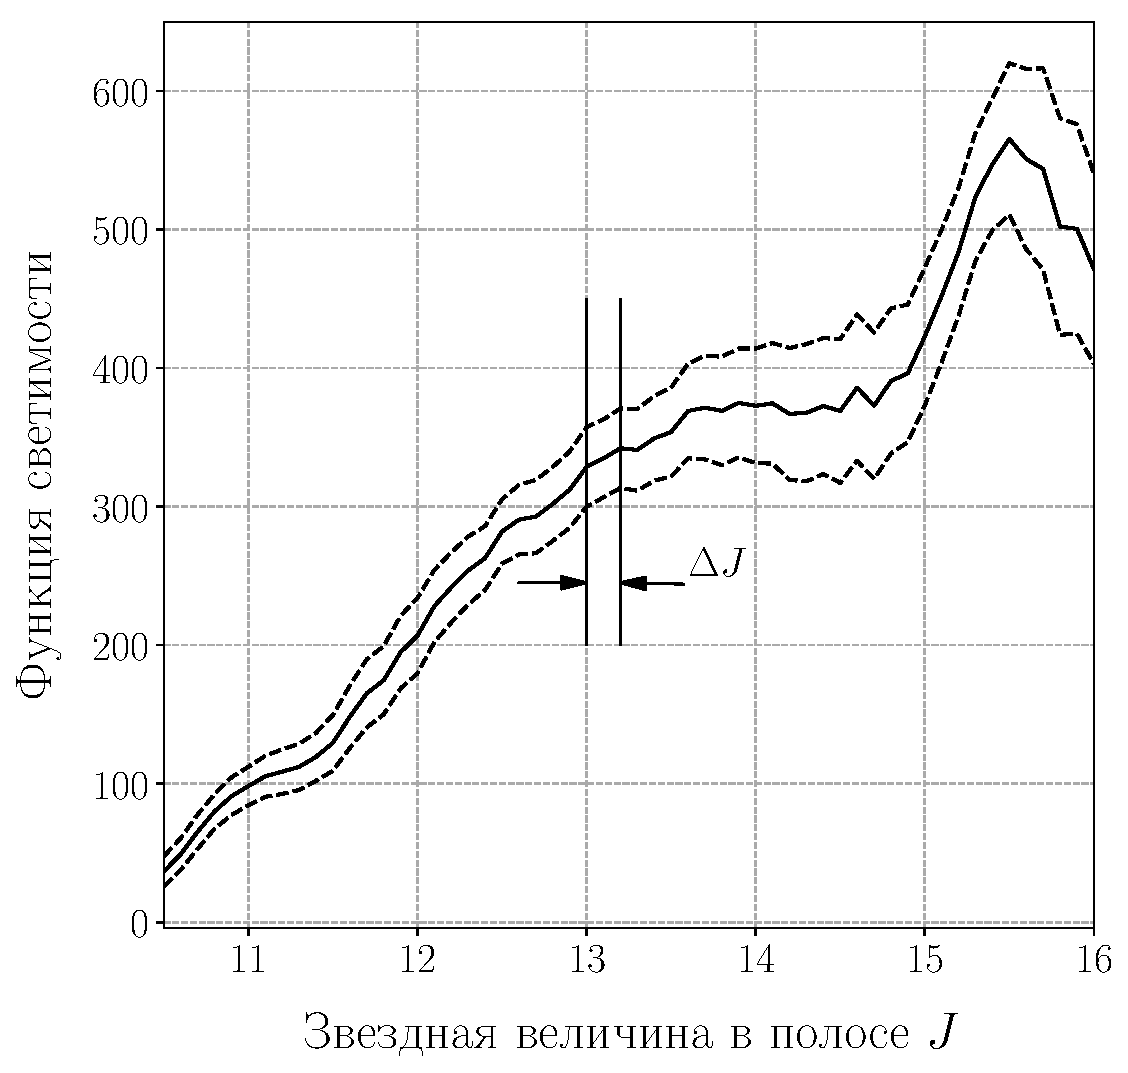
\includegraphics[width=7cm]{images/LF}
	\caption{Разбиение функции светимости (сплошная линия) скопления NGC 2099 на интервалы звездных величин. Пунктиром обозначен доверительный интервал функции светимости.}
	\label{LF}
\end{figure}

Затем мы переходим от звездной величины к массе, следующим образом. Сначала выбирается изохрона, которая соответствует возрасту скопления. Мы брали значение возраста из каталога Локтина и Поповой \cite{LoPo}, а затем уточняли, сравнивая с изохронами \cite{Bressan} диаграмму звездная величина-показатель цвета для отобранных звезд  скопления. Затем мы вычисляли абсолютные звездные величины, используя значения модуля расстояния и поглощения. Набор перечисленных параметров представлен в таблице \ref{clusters}. 

Зная абсолютную звездную величину звезд скопления, по таблице изохроны соответствующего возраста им можно сопоставить массы.  И теперь, с помощью формулы \ref{EkersEq} пересчитываем массу в значение светимости.

В таблицу \ref{clusters} также включили интервал масс, где минимальная масса соответствует звездной величине $J = 16^m$ (кроме скопления NGC 6834, для которого из-за недостаточной полноты каталога 2МАSS взята $J = 15.9^m$), а максимальная масса определяется звездами, которые находятся у точки поворота (для ее определения мы использовали главную последовательность нулевого возраста).


\begin{table}[h!]
\caption{Параметры функций светимости скоплений}
\vspace{0.5cm}
\centering
		\begin{tabular}{|c|c|c|c|c|}
			\hline
				{Скопление} & {Интервал по $M, M_{\odot}$}& ${(m-M)_0}$ & \ ${E(B-V)}$ & ${\log(t)}$\\
			\hline
			IC2714 & [0.73; 2.82] & 10.48 & 0.34 & 8.6\\
			NGC1912 & [0.68;  3.60] & 10.29 & 0.25 & 8.3\\
			NGC2099 & [0.76;  2.77] & 10.74 & 0.30 & 8.7\\
			NGC6834 & [1.07;  5.12] & 11.59 & 0.71 & 7.9\\
			NGC7142 & [0.87;  1.80] & 10.2 & 0.25 & 9.2\\
			\hline
		\end{tabular}
\label{clusters}
\end{table}

 Для каждой двойной системы из выбранного интервала звездных величин определяется свое отношение масс компонент двойной (параметр $q$) с помощью метода Неймана. Затем мы построим систему уравнений:
 
\begin{equation}
	\left\{
		\begin{aligned}
			&L=L_1+L_2\\
			&\log{L_1}= -0.705(\log{M_1})^2  + 4.655(\log {M_1}) - 0.025\\
			&\log{L_2}= -0.705(\log{M_2})^2  + 4.655(\log {M_2}) - 0.025\\
			&q=\frac{M_2}{M_1}\\
		\end{aligned}
	\right.\label{MAINsystem}
\end{equation}

где $L$ это светимость двойной (эта величина нам дана), а следующие величины являются неизвестными:
$L_1$ и $L_2 $ -- светимости компонентов двойной звезды,
$M_1$ и $M_2$ -- массы звезд-компонентов.

Для решения системы (\ref{MAINsystem}) введем следующие обозначения: заменим $\log{M_1}$ на $x$, как величину, которую требуется найти. Также для краткости обозначим постоянные коэффициенты буквенными символами: $a=-0.705 ,b=4.655, c=- 0.025$.

После ряда преобразований мы можем вывести формулу, в которой будет выражена суммарная светимость двойной звезды:

\begin{equation}
\ln{L} = \ln{10} (ax^2+bx+c)+\ln{(1 + exp(\ln{10}(a(\log {q})^2+\log {q}(b+2ax))))}
\end{equation}

Нашей целью является определить $x$, поэтому мы строим функцию $f(x)$, которая обращается в ноль при таком $x$, который является решением системы (\ref{MAINsystem}):

\begin{equation}
f(x)=\ln{10} (ax^2+bx+c)+\ln{(1 + exp(\ln{10}(a(\log {q})^2+\log {q}(b+2ax)))†)} - \ln{L}
\end{equation}

Чтобы решить данное уравнение, мы используем метод Ньютона. 
Для этого мы вычисляем значение $x_{k+1}=x_k - \sfrac{f(x_k)}{f'(x_k)}$ 
до тех пор, пока разница $|x_{k+1} - x_k|$ не примет требуемую точность (где $f'(x_k)$ -- производная функции $f(x)$ в точке $x_k$). 

Метод Ньютона имеет ограничения в использовании. Для того, чтобы процесс итераций сошелся, должны быть выполнены некоторые условия.

Во-первых, мы должны правильно выбрать начальную точку, которая будет находиться близко к корню уравнения. Для этого мы строим сначала цикл с маленьким шагом в интервалах значения искомой массы $[0.08 \mathfrak{M}_{\odot};10 \mathfrak{M}_{\odot}]$ (из физических соображений значения для главной компоненты двойной системы), то есть для $x \in [-1.1,1.0]$. Цикл заканчивает свою работу, когда находит такое значение $x_i$, для которого $f(x_i)\cdot f(x_{i+1}) <0$. Это значит, что корень уравнения находится в интервале $x \in [x_i,x_{i+1}]$. Таким образом, мы считаем, что $x_i$ это и есть стартовая точка метода Ньютона.

Во-вторых, функция $f(x)$ должна быть непрервыной в области поиска нашего корня. Этот факт легко доказывается, так как $f(x)$ является комбинаций непрерывных на данном интервале $x$ функций, а именно: экспоненциальной, логарифмической, квадратичной.

Полученное в ходе решения уравнения методом Ньютона $x_k$ будет корнем уравнения, следовательно масса $M_1=10^x$ будет искомой массой главной компоненты двойной из системы уравнений (\ref{MAINsystem}).
Затем мы можем восстановить массу второй компоненты двойной по известному коэффициенту $q$, а затем и полную массу системы $M_1+M_2$.

Мы должны повторить данную процедуру для всех $N_{b}$  звезд и определить массу двойных в интервале звездных величин $\Delta J$, а затем просуммировать эти значения для всех интервалов, чтобы узнать массу двойных в скоплении.

После этого, чтобы получить массу скопления, нам нужно определить массу оставшихся одиночных звезд в количестве $N-N_{b}$ в каждом интервале $\Delta J$. Для определения массы звезды мы пользуемся таблицей изохроны, в которой приведены значения масс в соответствии с абсолютной звездной величиной. Отсюда и получаем массу всего скопления с учетом двойных звезд:

\begin{equation}
M_{clb} = M_{b}+M{s}
\end{equation}

Для определения разброса решения данный алгоритм был проведен 30 раз, чтобы получить некоторый набор значений масс. Конечным результатом стали среднее значение и величина дисперсии. Источником разброса значений масс скопления является статистическое определение параметра $q$ из заданного распределения. При фиксированном $q=1$ случайная ошибка равна 0.

Чтобы сравнить массу скоплений с учетом двойных $M_{clb}$ с массой скопления, состоящего только из одиночных звезд, $M_{wob}$, необходимо получить $M_{s}$ из всех данных нам звезд. Это значит, нужно воспользоваться нашим алгоритмом со значением $\alpha = 0$.

\section*{Результаты}

В этой работе мы использовали функции светимости пяти рассеянных звездных скоплений IC 2714, NGC 1912, NGC 2099, NGC 6834 и NGC 7142.

Мы рассмотрели два варианта случая одинаковых масс компонент.  В первом случае рассматриваем только двойные звезды. Во втором случае мы также учитываем кратные системы (тройной и четверной кратности) в численном соотношении согласно работе А. Токовинина \cite{Tokovinin}. В ней было определено, что системы кратностей 1:2:3:4:5 (1 означает одиночную звезду) имеют относительную численность 54:33:8:4:1.

На рисунке \ref{results_g} показана зависимость поправочного коэффициента от доли двойных в разных предположениях вида распределения параметра $q$. Сразу же видно, что поправки в случаях равных масс компонент явно превышают поправки при других моделях.

\begin{figure*}[h!]
	\centering
	\begin{multicols}{3}
	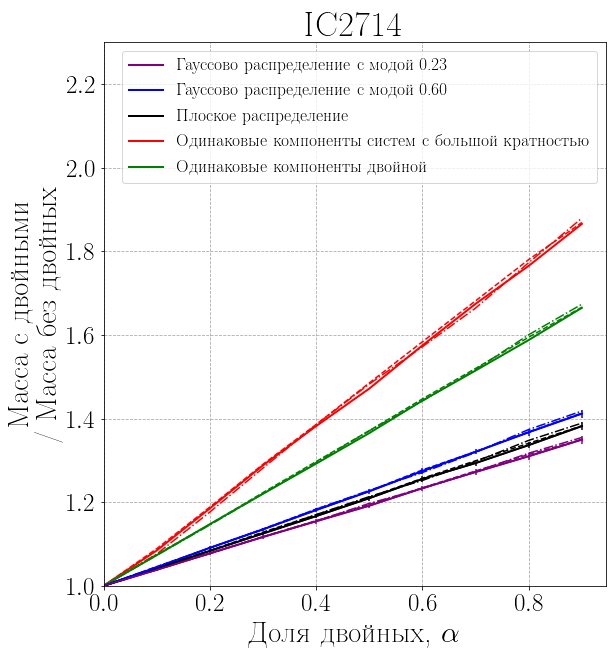
\includegraphics[width=5cm]{images/alphas_IC2714}
	\columnbreak
	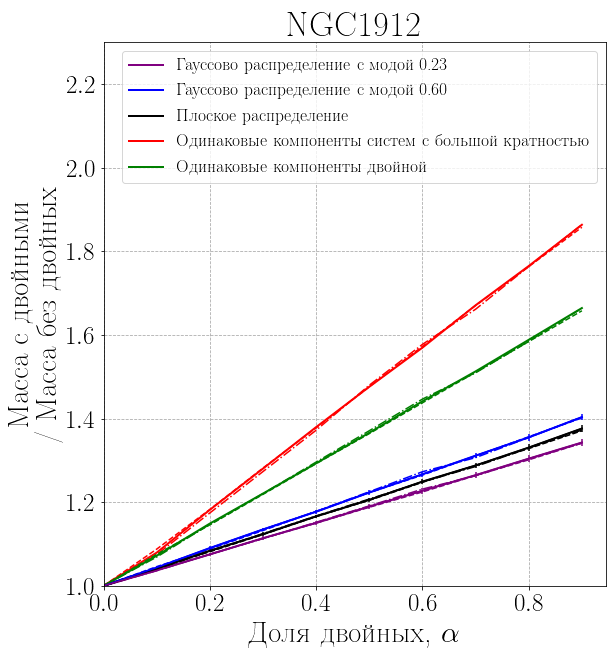
\includegraphics[width=5cm]{images/alphas_NGC1912}
	\columnbreak
	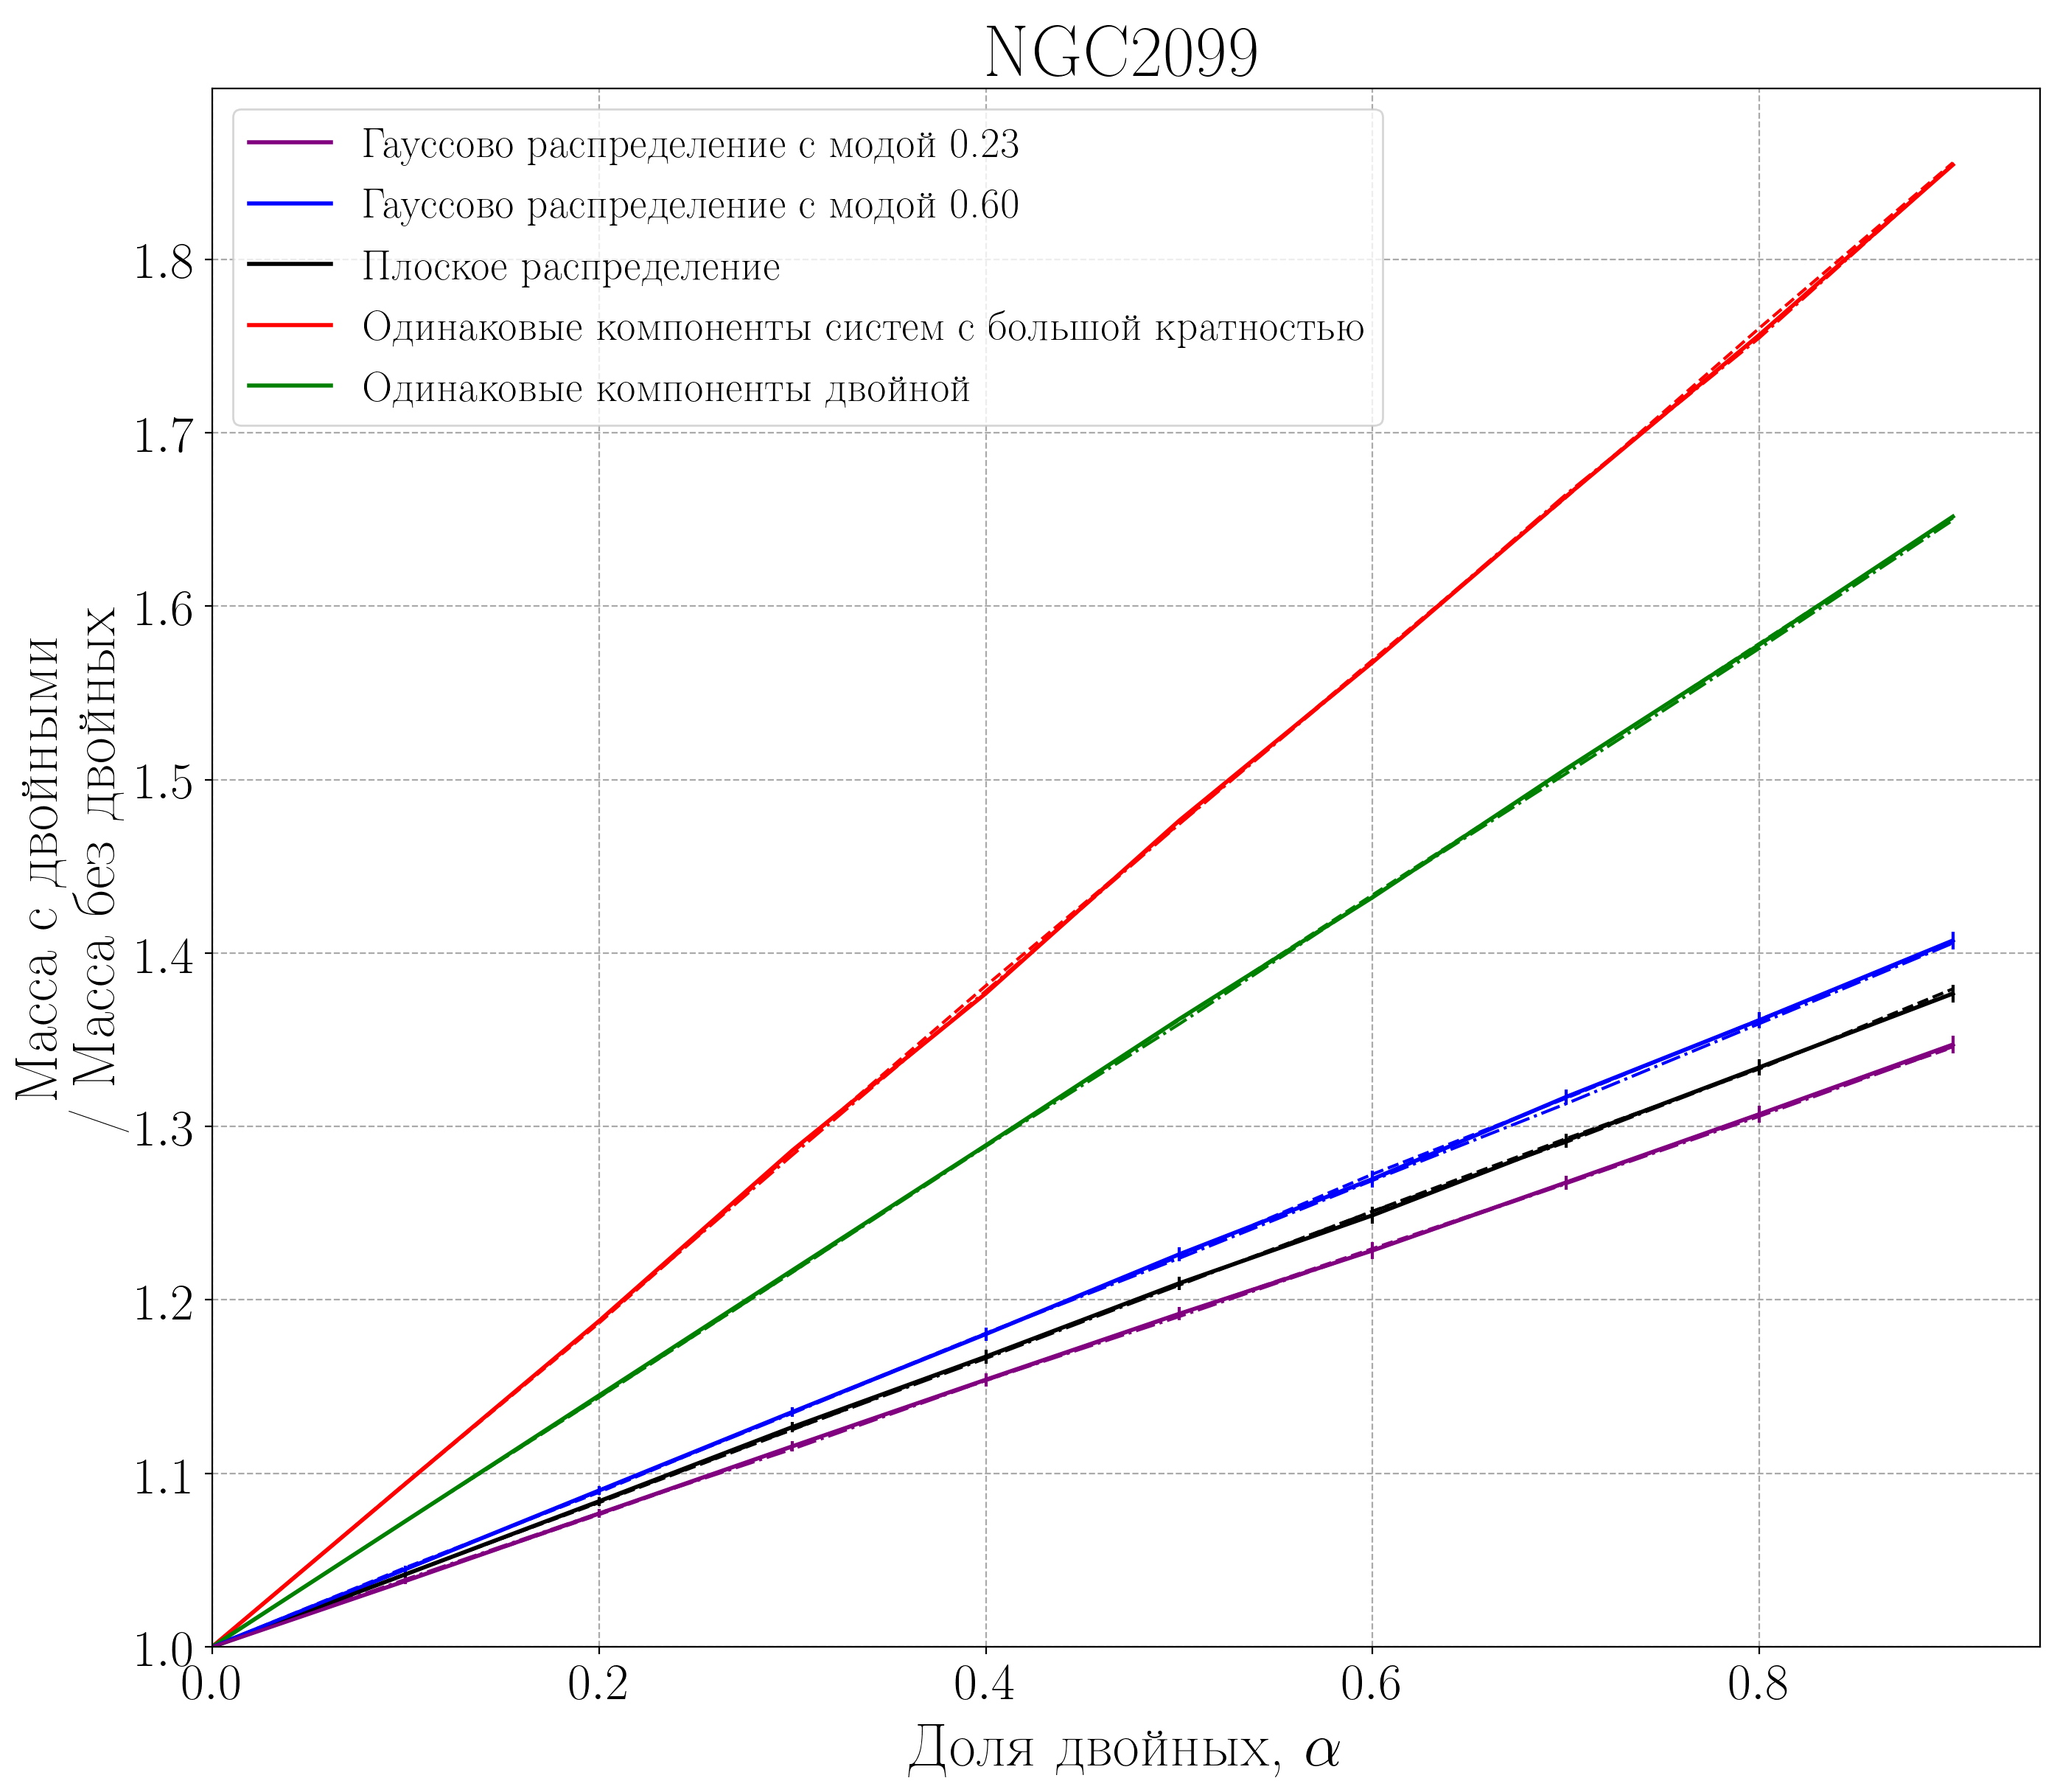
\includegraphics[width=5cm]{images/alphas_NGC2099}
	\end{multicols}
	
	\begin{multicols}{2}
	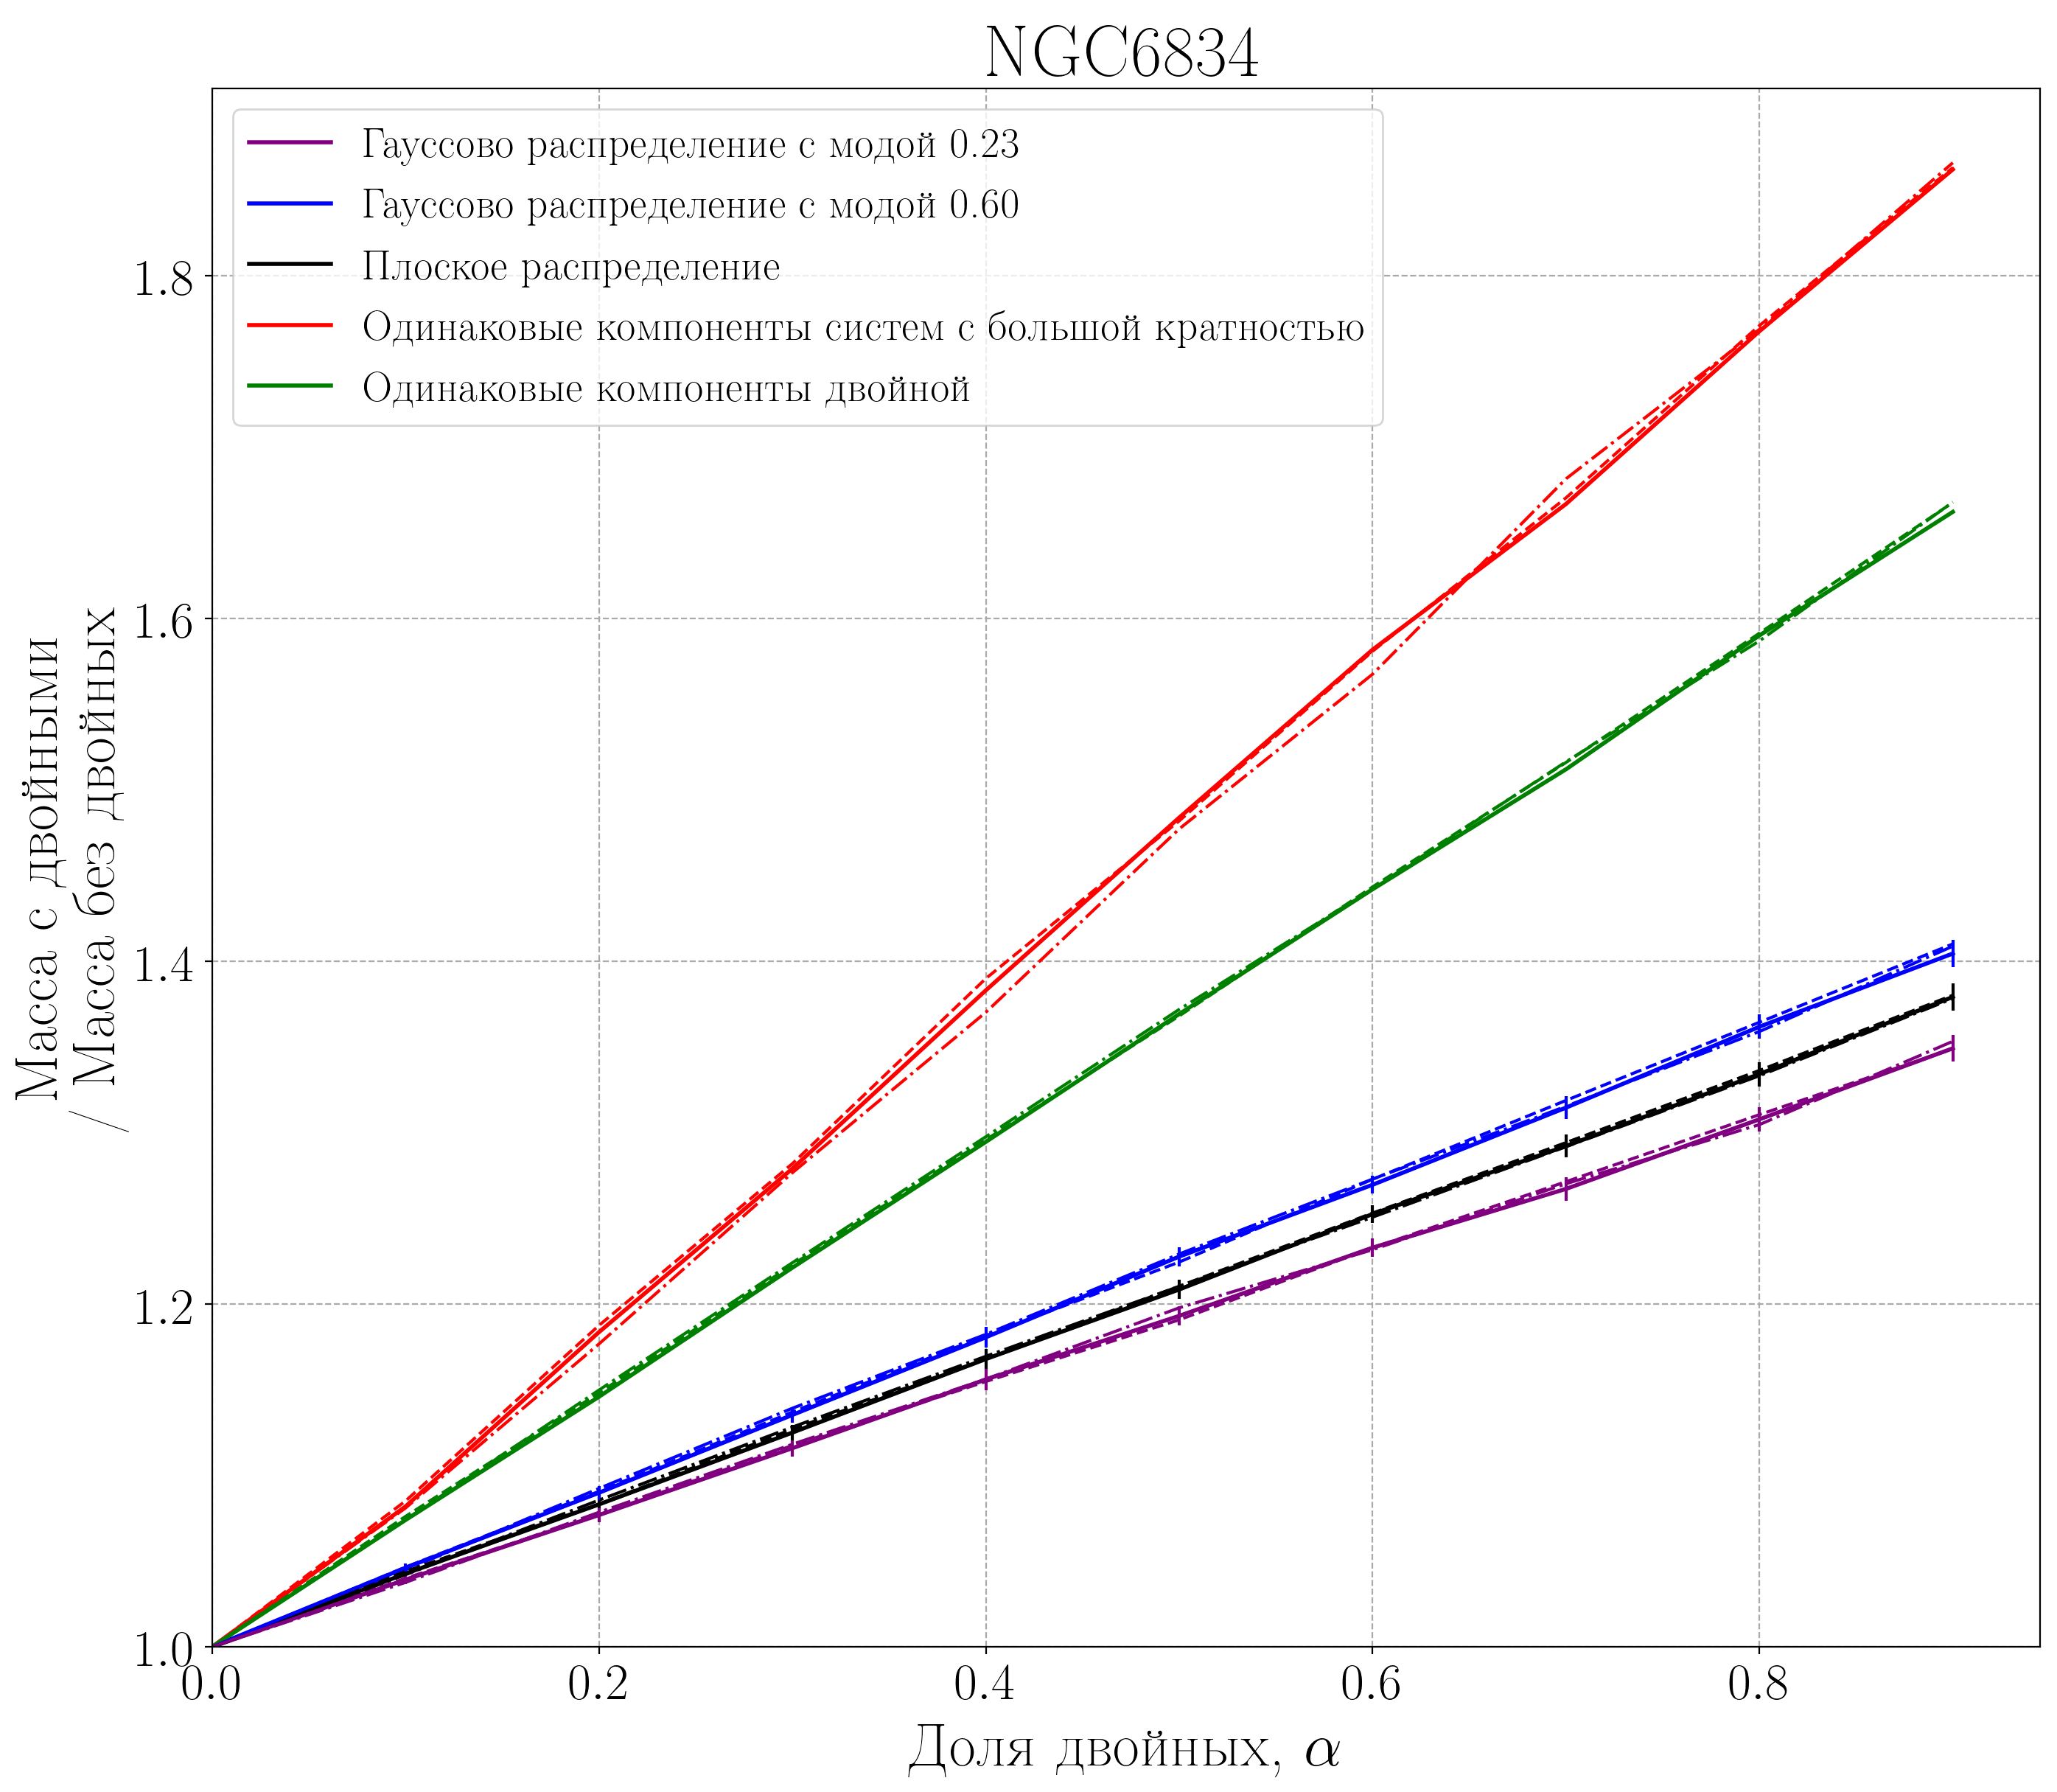
\includegraphics[width=5cm]{images/alphas_NGC6834}
	\columnbreak
	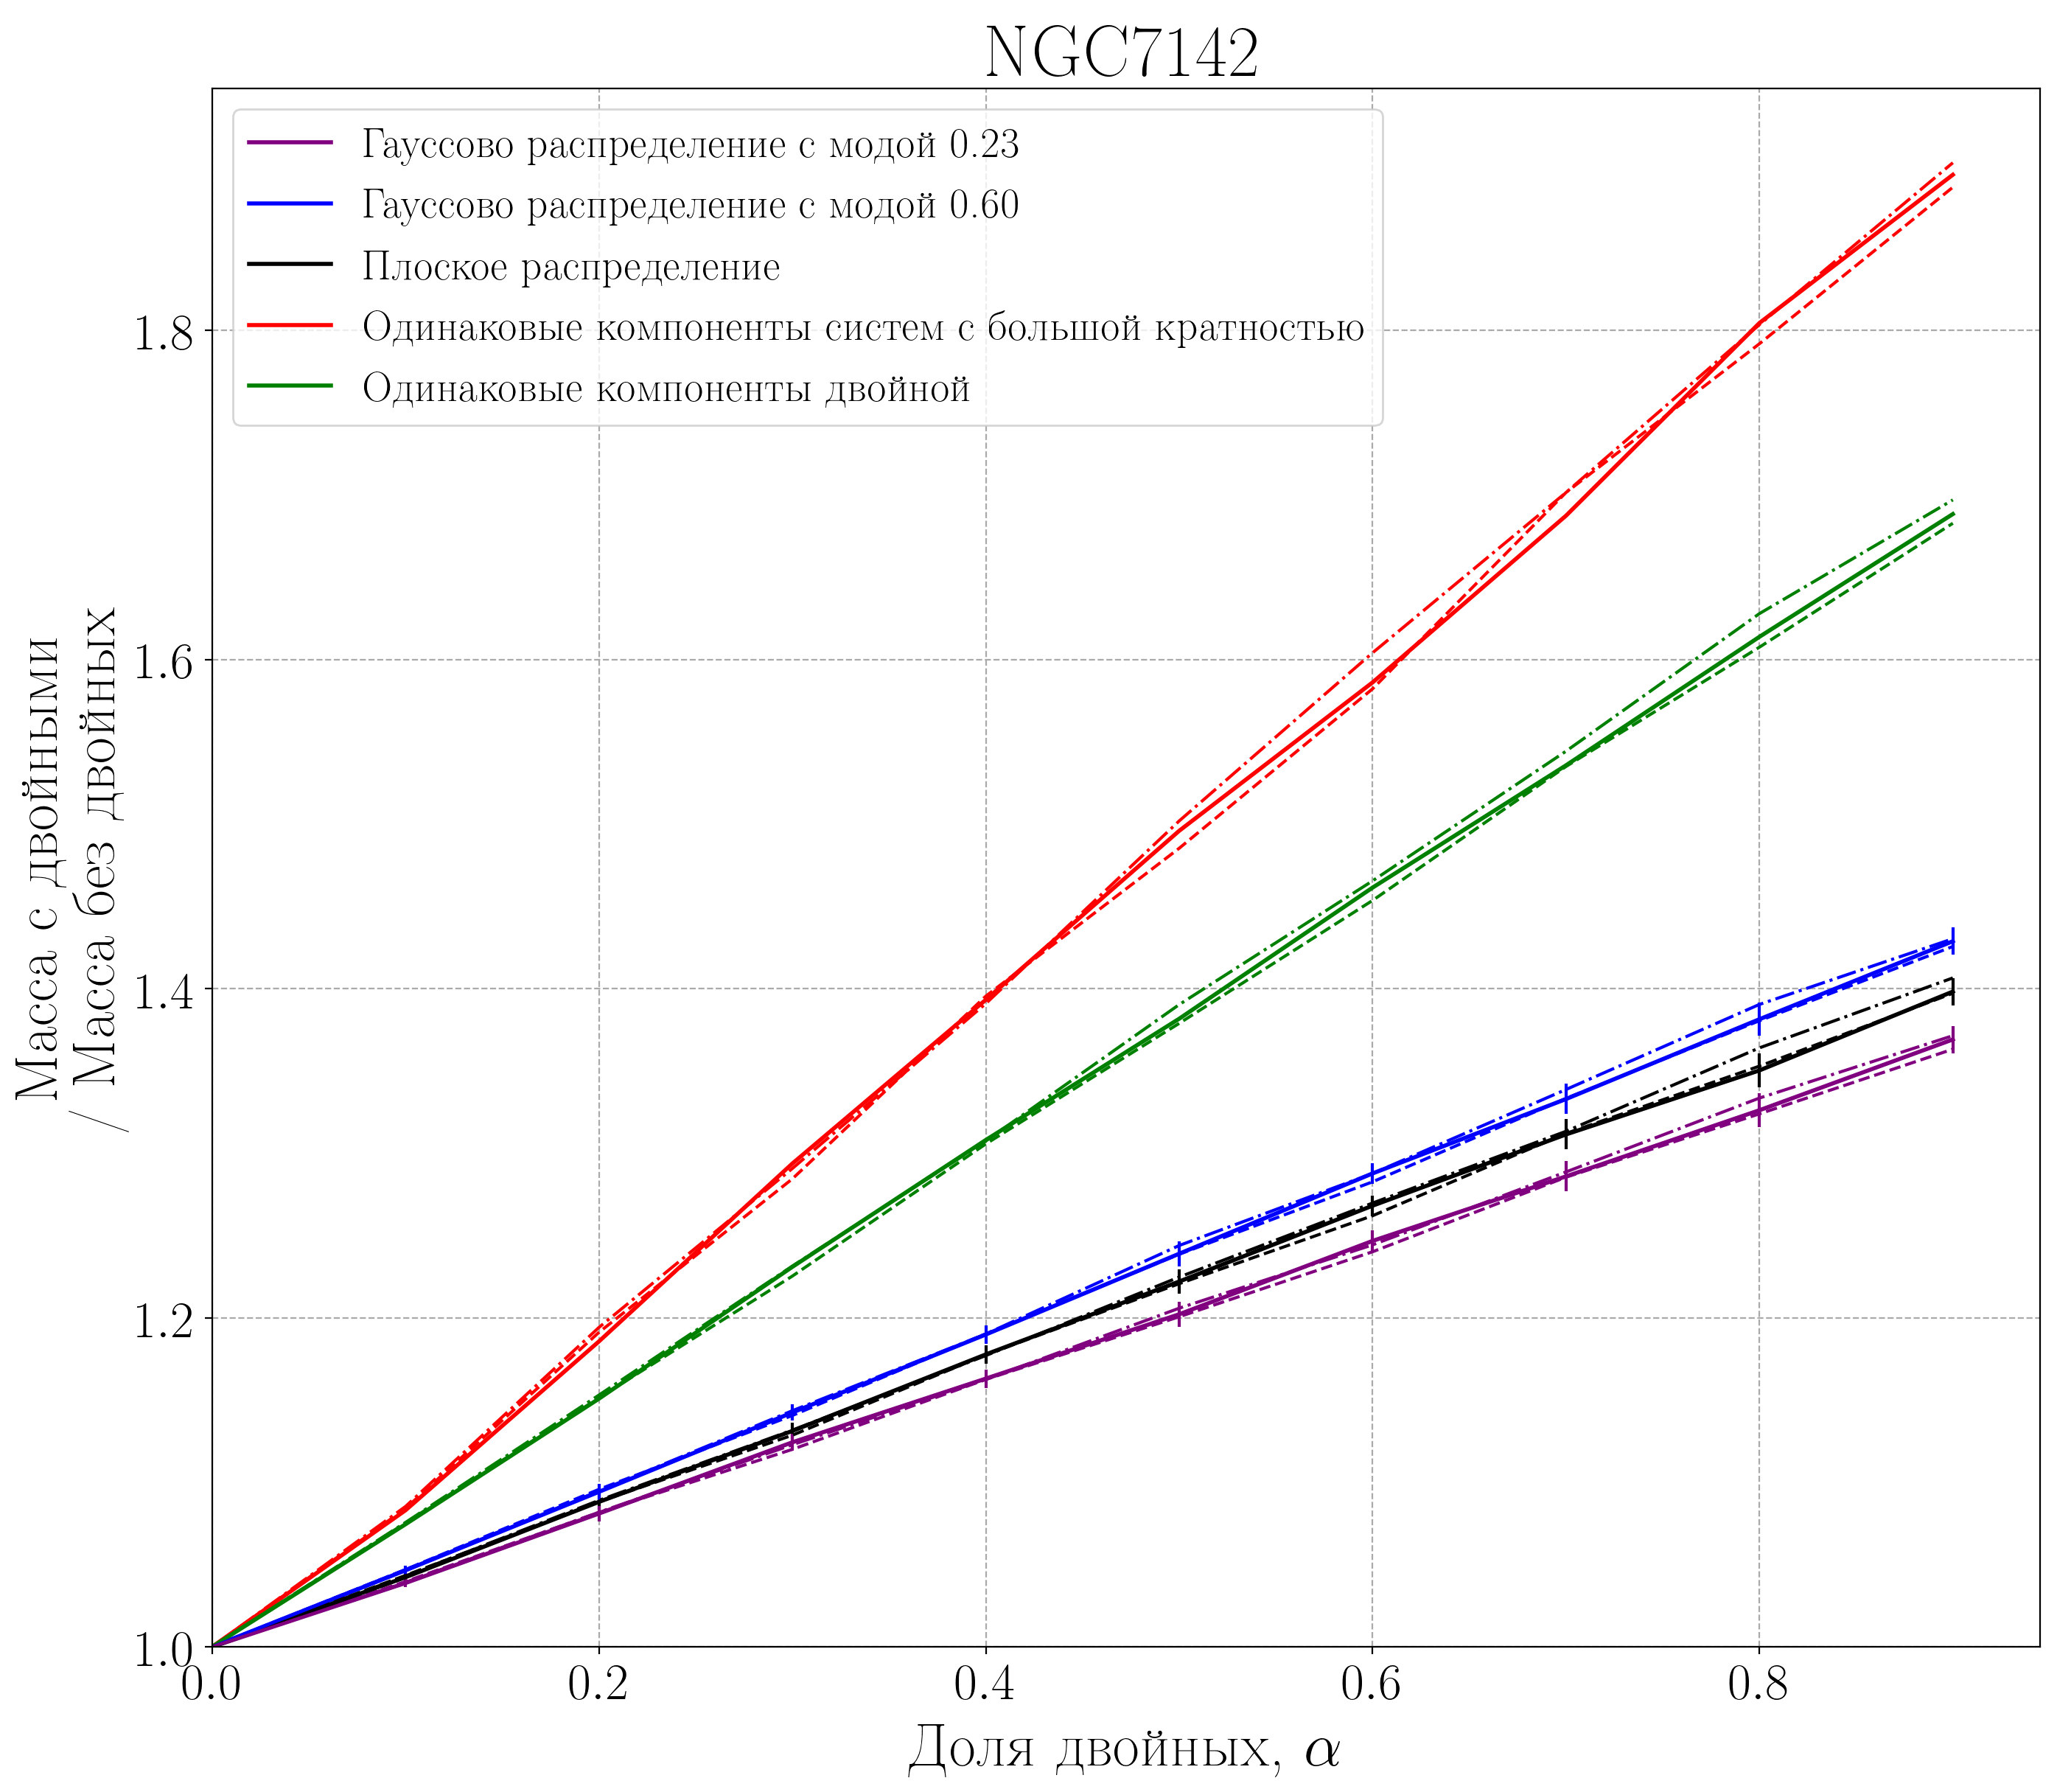
\includegraphics[width=5cm]{images/alphas_NGC7142}

	\end{multicols}
	\caption{Зависимость поправочного коэффициента от доли двойных в разных предположениях вида распределения параметра $q$}
	\label{results_g}
\end{figure*}

Khalaj \& Baumgardt \cite{Khalaj} в своей работе определили, что для доли двойных, равной 0.35, поправочный коэффициент к массе скопления равен 1.35. Согласно нашему исследованию для данной доли поправка к массе принимает значения в промежутке между 1.10 и 1.15 в случае реалистичных распределений. Однако, если учесть возможное наличие систем большей кратности, то поправка к массе скопления достигает 1.32 в случае одинаковых компонент. Мы применили линейную регрессию к полученным зависимостям и привели результаты в таблице (\ref{results_t}). В данной таблице представлена следующая информация: модель распределения по $q$ и название скопления, коэффициенты $A$ и $B$ линейной регрессии $y = A + B\alpha$ (где $y$ это поправка к массе, а $\alpha$ – доля двойных звезд), ${\chi ^2}$ аппроксимации  и параметр адекватности модели $Q$(\cite{Press}). Коэффициенты $A$ практически во всех случаях можно считать равными 1. Для любого выбранного реалистического распределения коэффициенты $B$ имеют одинаковые значения в пределах ошибки (кроме самого старого скопления -- NGC 7142). Из этого следует, что функция светимости не влияет значительным образом на значение поправки к массе скопления за счет учета неразрешенных двойных.

\begin{table}[h!]
\caption{Параметры линейной регрессии $y = A + B\alpha$ для зависимости поправочного коэффициента к массе от доли двойных}
\vspace{0.5cm}
\centering
		\begin{tabular}{|c|c|c|c|c|c|}
			\hline
				{Распределение по $q$} & {Скопление}& ${A}$ & ${B}$ & ${\chi ^2}$ & {Q}\\
			\hline
				Одинаковые  &IC 2714&$1.000 \pm 0.002$&$0.736 \pm 0.005$&0.673&1.000\\
				компоненты &NGC 1912&$1.000 \pm 0.002$&$0.735 \pm 0.005$&1.162&0.997\\
				двойных&NGC 2099&$1.000 \pm 0.000$&$0.722 \pm 0.001$&1.639&0.990\\
					&NGC 6834&$1.000 \pm 0.002$&$0.736 \pm 0.007$&1.025&0.998\\
					&NGC 7142&$0.997 \pm 0.001$&$0.773 \pm 0.006$&1.263&0.996\\
			\hline
				Одинаковые  &IC 2714&$0.994 \pm 0.005$&$0.968 \pm 0.012$&1.690&0.989\\
				компоненты &NGC 1912&$0.991 \pm 0.004$&$0.968 \pm 0.006$&2.316&0.970\\
				звезд разной&NGC 2099&$0.999 \pm 0.000$&$0.949 \pm 0.001$&5.274&0.728\\
				кратности&NGC 6834&$0.987 \pm 0.003$&$0.975 \pm 0.005$&5.582&0.694\\
					&NGC 7142&$0.983 \pm 0.003$&$1.020 \pm 0.007$&6.496&0.592\\
			\hline
				Плоское &IC 2714&$0.999 \pm 0.004$&$0.423 \pm 0.011$&0.181&1.000\\
				распределение &NGC 1912&$1.000 \pm 0.004$&$0.414 \pm 0.009$&0.227&1.000\\
				&NGC 2099&$1.000 \pm 0.002$&$0.417 \pm 0.005$&0.194&1.000\\
					&NGC 6834&$1.000 \pm 0.003$&$0.419 \pm 0.008$&0.185&1.000\\
					&NGC 7142&$0.998 \pm 0.004$&$0.447 \pm 0.011$&0.190&1.000\\
			\hline
				Гауссово &IC 2714&$1.000 \pm 0.004$&$0.389 \pm 0.010$&0.086&1.000\\
				распределение &NGC 1912&$0.999 \pm 0.004$&$0.381 \pm 0.009$&0.061&1.000\\
				с модой $\mu = 0.23$&NGC 2099&$1.000 \pm 0.003$&$0.384 \pm 0.006$&0.273&1.000\\
					&NGC 6834&$1.000 \pm 0.003$&$0.386 \pm 0.008$&0.256&1.000\\
					&NGC 7142&$0.998 \pm 0.004$&$0.411 \pm 0.010$&0.167&1.000\\
			\hline
				Гауссово &IC 2714&$0.998 \pm 0.003$&$0.389 \pm 0.010$&0.218&1.000\\
				распределение &NGC 1912&$1.000 \pm 0.004$&$0.381 \pm 0.009$&0.265&1.000\\
				с модой $\mu = 0.60$&NGC 2099&$1.000 \pm 0.002$&$0.384 \pm 0.006$&0.073&1.000\\
					&NGC 6834&$1.001 \pm 0.003$&$0.386 \pm 0.008$&0.161&1.000\\
					&NGC 7142&$0.999 \pm 0.003$&$0.411 \pm 0.010$&0.058&1.000\\
			\hline
		\end{tabular}
\label{results_t}
\end{table}
 
Функции светимости, которые мы использовали в нашей работе, ограничены по видимой звездной величине ввиду неполноты каталога 2MASS. По этой причине мы не можем рассматривать массы ниже, чем минимальное значение интервала из таблицы (\ref{clusters}). Поэтому стоит выяснить, как это ограничение влияет на результат. Мы изначально сделали предположение, что доля двойных $\alpha$ не зависит от звездной величины. В таком случае поправка к массе скопления теоретически не должна зависеть от того, какие мы рассматриваем границы по звездным величинам для скоплений. Чтобы подтвердить нашу гипотезу, мы проделали следующий эксперимент. Для скопления NGC 2099 мы посчитали поправочный коэффициент к массе для набора максимальных звездных величин: $J_{lim} = 14^m, 15^m, 16^m$ для случая плоского распределения. Оказалось, что поправочный коэффициент слабо растет с ростом лимитирующей звездной величины. Например, для доли двойных $\alpha = 0.8$ $y = 1.322 \pm 0.013$ для $J_{lim} = 14^m$, $y = 1.328 \pm 0.009$ для $J_{lim} = 15^m$, и $y = 1.334 \pm 0.006$ для $J_{lim}  = 16^m$.


Если доля двойных растет с ростом звездной величины, поправочный коэффициент к массе тоже будет расти со звездной величиной. Если доля двойных снижается с ростом звездной величины, можно ожидать, что поправочный коэффициент будет независим от звездной величины, или даже будет снижаться.
В любом случае, стоит подчеркнуть, что при использовании поправочного коэффициента нельзя найти полную массу скопления, а только лишь улучшить нижнюю оценку его массы.

\section*{Заключение}

В этой работе мы попытались определить увеличение оценки массы скопления, полученной путем звездных подсчетов, за счет учета неразрешенных звезд. Полученные графики представлены на рисунке \ref{results_g} и в таблице 

Самые важные результаты данного исследования следующие:

\begin{itemize}
	\item Зависимость поправки к массе скопления от доли двойных является линейной во многих случаях.
	\item Зависимость поправки к массе скопления от доли двойных значительно не отличается для реалистичных распределений параметра $q$: двух Гауссовых распределения с модами $\mu_q = 0.23$ и $\mu_q = 0.60$ и плоского распределения. Из таблицы и графиков \ref{results_g} видно, что чем ближе максимум распределения к 1, тем больше поправочный коэффициент.
	\item Зависимость поправки к массе скопления от доли двойных для выбранного распределения существенно не отличаются (за исключением самого старого скопления NGC 7142). Поэтому можем считать, что вид функции светимости значительно не влияет на значение поправчного коэффициента
	\item Для частного случая доли двойных $\alpha =0.35$  поправка к массе скопления может принимать значения между 1.10 и 1.15 для реалистичных распределений. Однако, если учитывать наличие кратных систем (тройные звезды и т.д.), поправка возрастает (ее среднее значение 1.32 для случая одинаковых компонент). Тогда оценка значения 1.35 для поправки к массе скопления Ясли, полученное Khalaj \& Baumgardt \cite{Khalaj} является допустимой.

\end{itemize}

Наши результаты помогут улучшить оценки массы скоплений, содержащих неразрешенные двойные звезды в широком диапазоне доли двойных и с различными предположениями о виде распределения отношения масс компонент $q$.

	\newpage
	\bibliography{Biblyo.bib}
\end{document}
